\chapter{Appendix}

\section{Unused plots}
\label{App:Plots}
\begin{figure}[H]
    \centering
    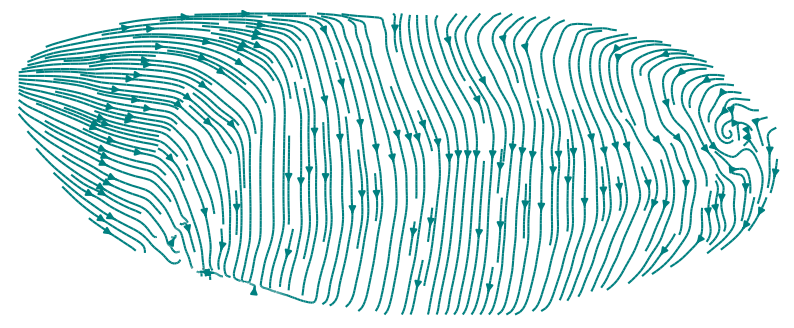
\includegraphics[width=1\linewidth]{chapters/Appendix/streamplot1.png}
\end{figure}

\begin{figure}[H]
    \centering
    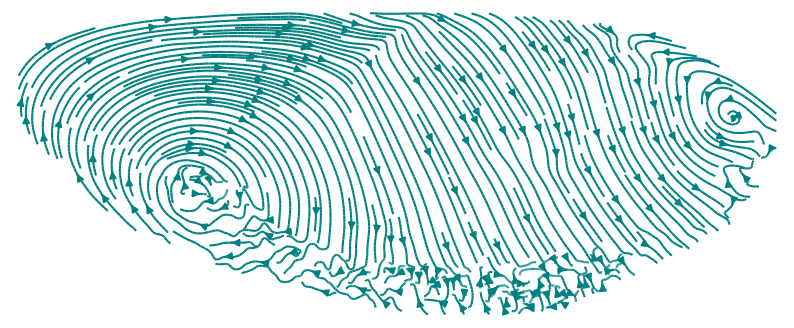
\includegraphics[width=1\linewidth]{chapters/Results/figures/streamplot2.png}
    \caption{
Without any basis of comparison this flow-field is not easy to interpret, but it looks cool.}
    \label{fig:streamplot}
\end{figure}


\begin{figure}[H]
    \centering
    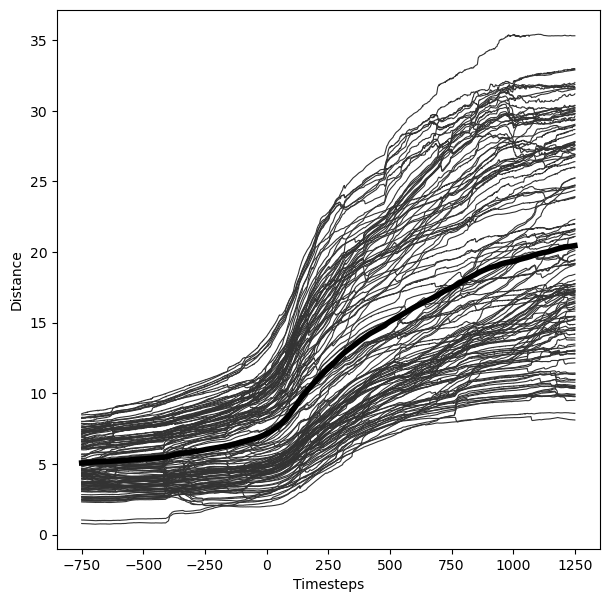
\includegraphics[width=1\linewidth]{chapters/Appendix/germbandMovementQuant.png}
    \caption{Horizontal-position of a line of germ-band cells, mirroring the analysis in  \url{https://www.ncbi.nlm.nih.gov/pmc/articles/PMC2801059/}}
    \label{fig:enter-label}
\end{figure}
\begin{figure}[H]
    \centering
    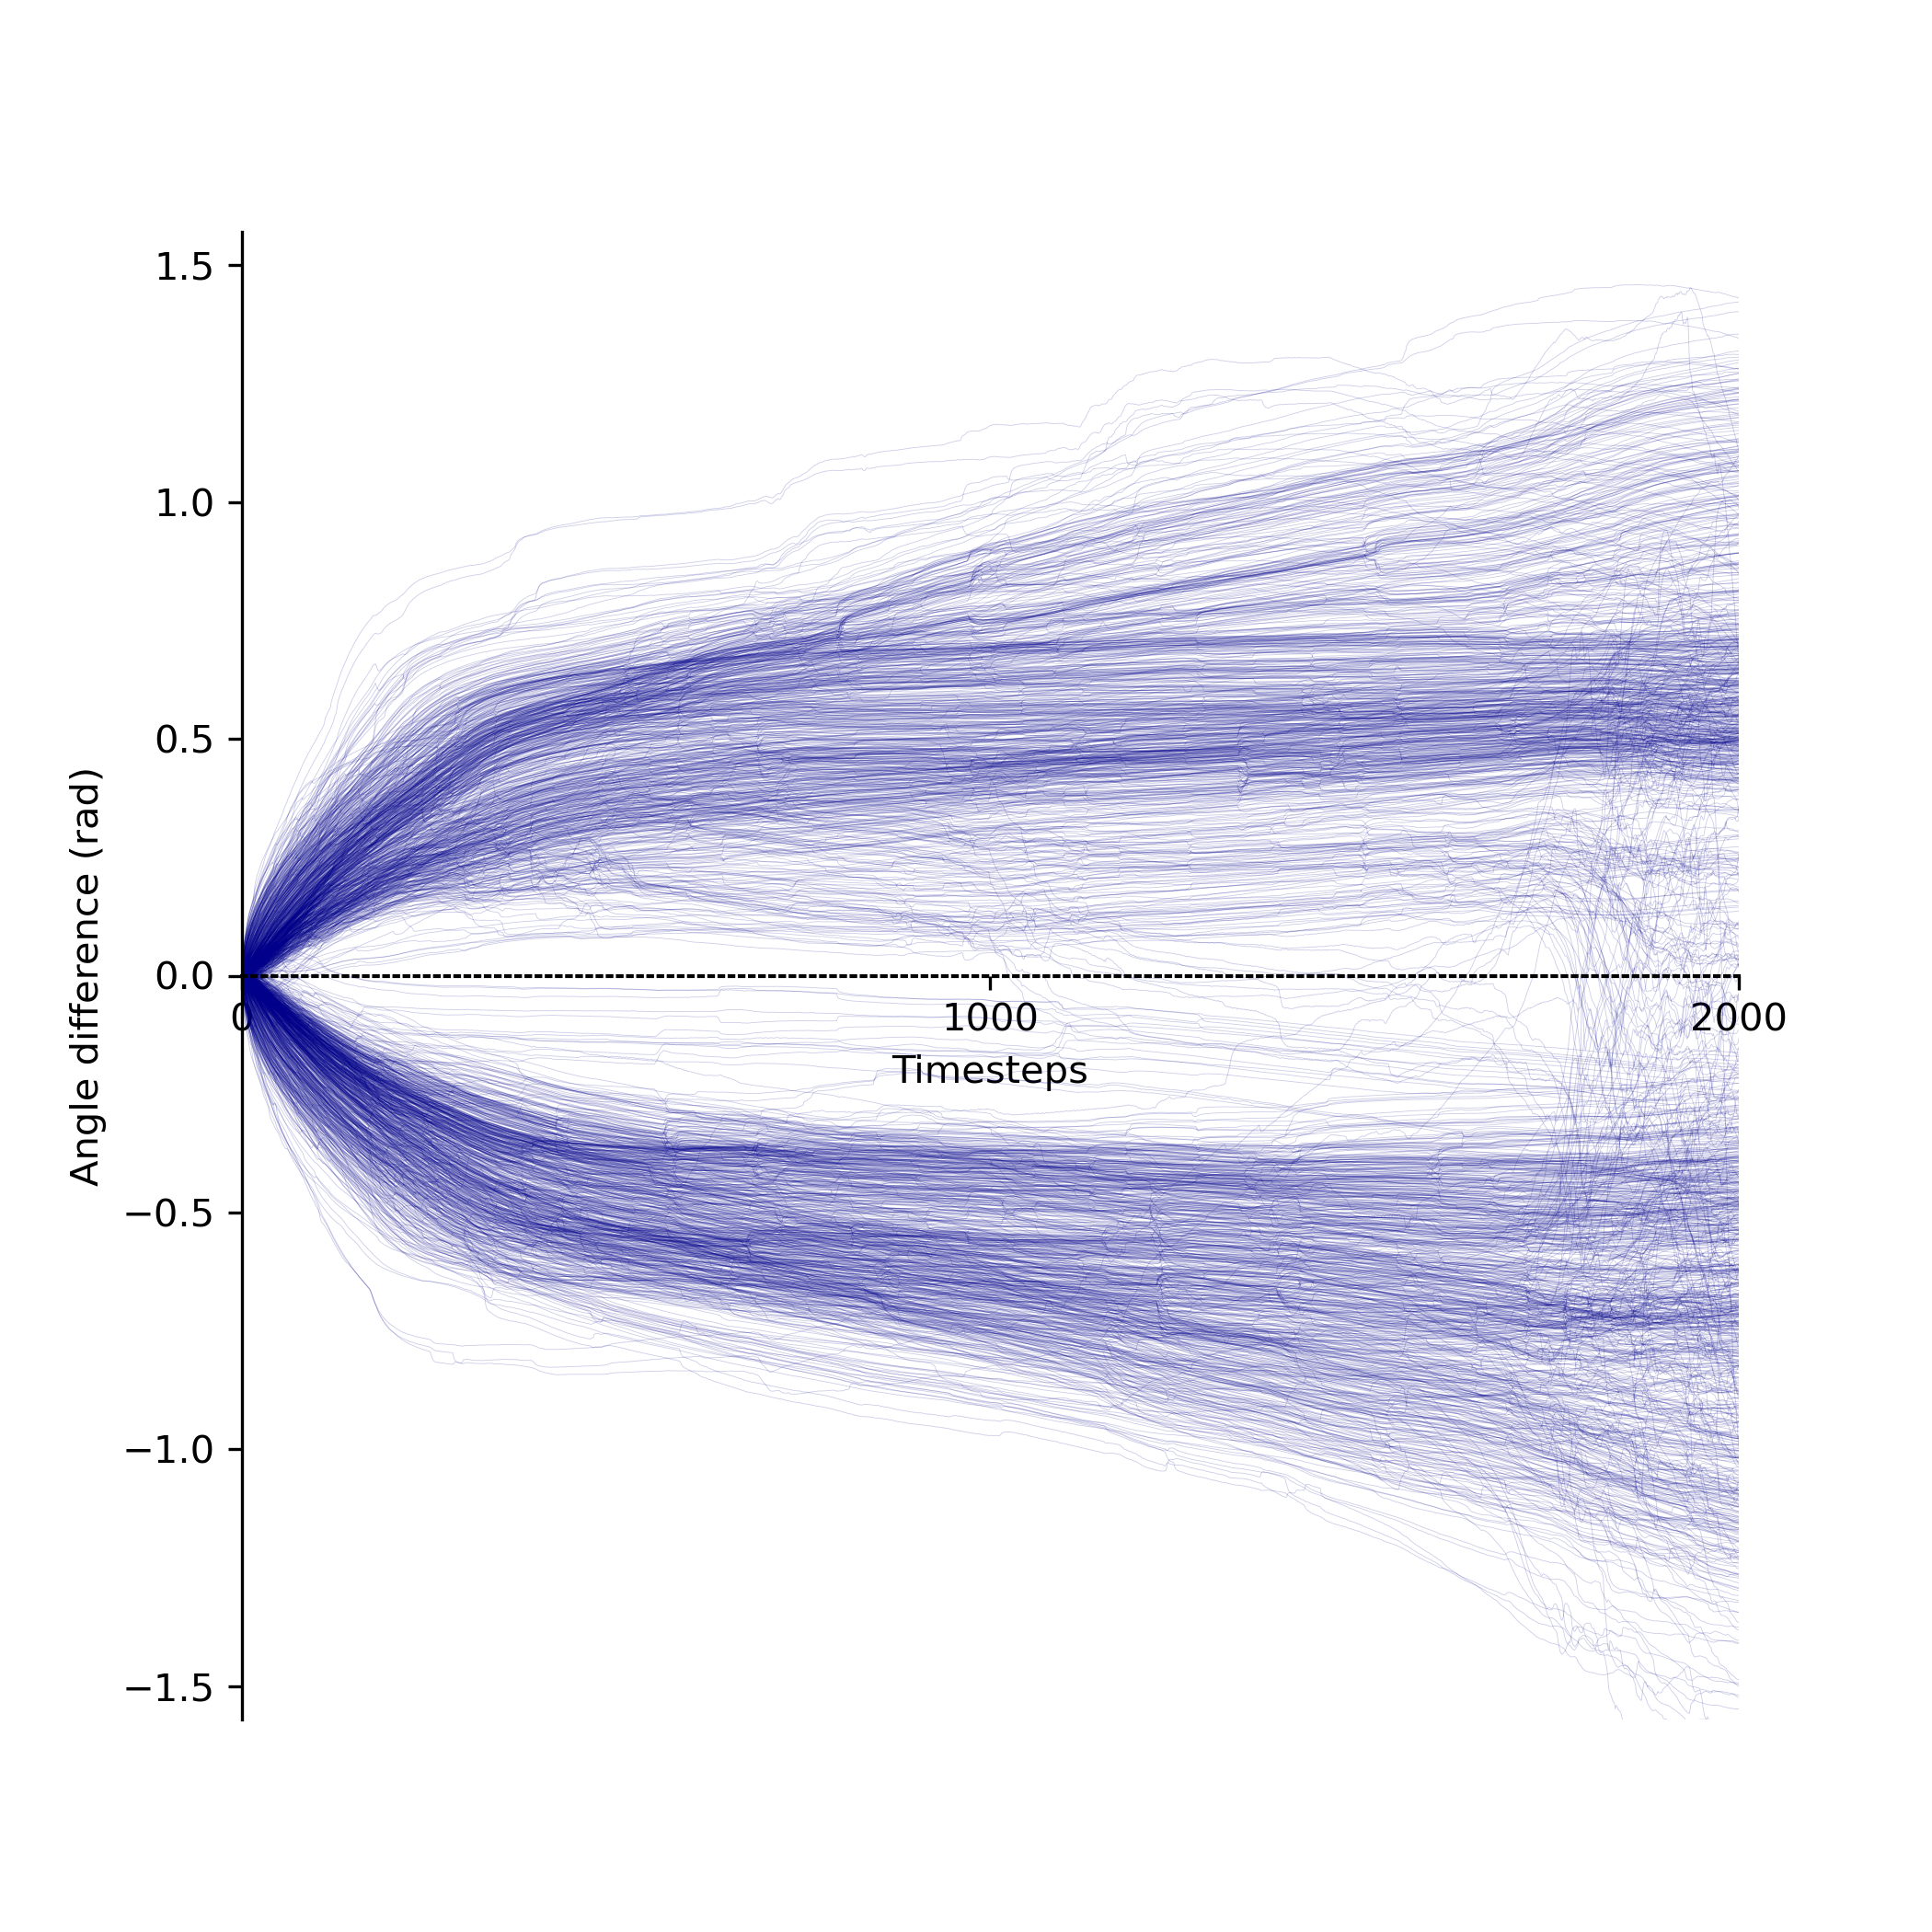
\includegraphics[width=1\linewidth]{chapters/Appendix/the_ring.png}
    \caption{Angle in cylindrical coordinates of germ-band. Mirroring \url{https://www.ncbi.nlm.nih.gov/pmc/articles/PMC2801059/}}
    \label{fig:enter-label}
\end{figure}
\section{Parameter Sensitivity Analysis}
No good examination of a model is complete without a Parameter Sensitivity Analysis:
\begin{figure}[H]
    \centering
    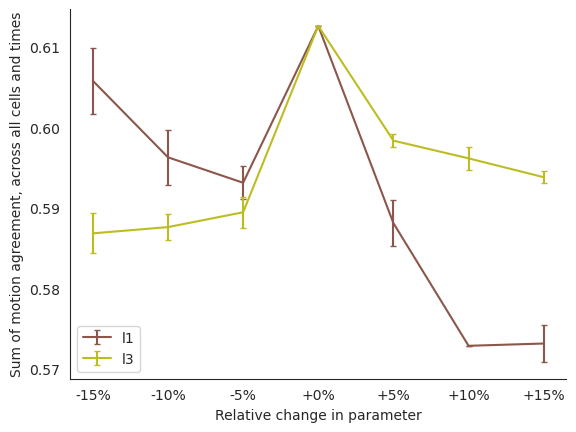
\includegraphics[width=0.8\linewidth]{chapters/Results/figures/PSA.png}
    \caption{The sum of the $\Delta$-metric as described in the results section. Error bars are mean and standard deviations of two runs using identical parameters but different seeds. }
    \label{fig:enter-label}
\end{figure}

In general, the solution is quite stable for perturbations to the two main parameters $\lambda_1$ and $\lambda_3$.

As can be seen, having a too high $\lambda_1$ lowers the internal pressure and therefore deforms the embryo and changes the timing. Lowering $\lambda_1$ seems to not be too bad, but the increased pressure exaggerates all invaginations quite dramatically.

Modifying $\lambda_3$ causes more understandable changes to the morphology (the error bars are also smaller). This comes down to the fact that $\lambda_3$ simply changes the pushing force of the germ-band during its elongation (\gb{A2}). Any change messes up the timing in its interactions with \vf{A1} and \pmg{A3}. In reality, the embryo has some self-correcting effects our model does not capture.




\section{Ventral Furrow}
\label{App:VF}
\begin{figure}[H]
    \centering
    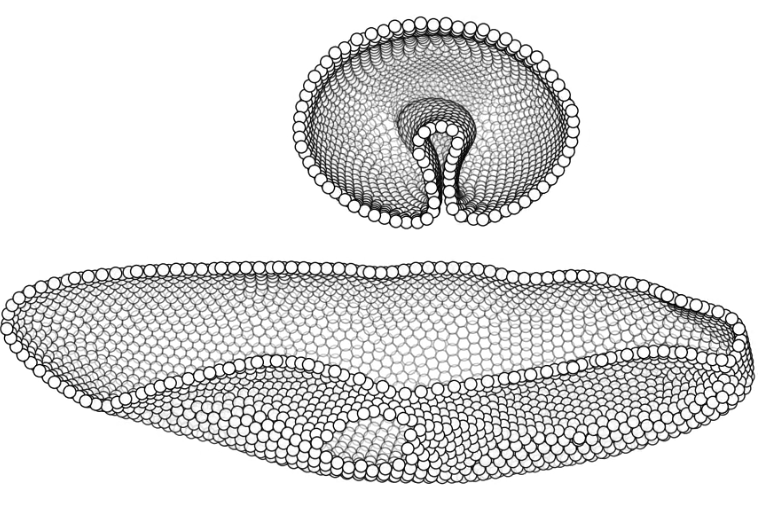
\includegraphics[width=0.9\linewidth]{chapters/Appendix/cross_sections.png}
    \caption{Just before the posterior midgut invaginates (\pmg{A3}). As can be seen, the ventral furrow, which is supposed to go no further than halfway up extends too much into the embryo. \\Note: The apparent hole in the internalized furrow is an artifact of cutting the cells in a plane.}
    \label{fig:enter-label}
\end{figure}
\section{Code details}
\label{App:Code}
By far the heaviest load, so optimizing this is the highest priority. Firstly, new neighbours are only found every 50th time step. 
Secondly, the search space is reduced by querying using SciPy's \verb|cKDTree|.
Finally, Voronoi neighbors are changed to "approximate line of sight neighbors" giving phenomenologically the same results while being magnitudes faster to calculate. The algorithm can be seen below:

\begin{lstlisting}
# dx = direction vectors
# d = distances
# n_neighbors = 0 for nearest neighbors, 1 for neareast and second nearest, and so on 


# Calculate pairwise midpoints between the cells
n_dis = torch.sum((dx[:, None, :] / 2 - dx[None, :, :]) ** 2, dim=3)

# add a large constant to the diagonal for no self-intersections 
n_dis += 1000 * torch.eye(n_dis.shape[1])[None, :, :]

# Find all cells that are closer than halfway to any other.
#    this effectively finds Voronoi neighbors.
z_mask = torch.sum(n_dis < (d[:, :, None] ** 2 / 4), dim=2) <= n_neighbors
\end{lstlisting}

The rest of the code base can be found on:
\url{https://github.com/JakobSchauser/Thesis/}
\section{Videos}
\label{App:videos}
The videos of the different simulated mutants can be found here:

\url{https://github.com/JakobSchauser/Thesis/tree/main/FinalVideos/Mutants/}
% \section{Sergei-analyses (tie into PCP)}
% \label{App:Sergei}

\section{Green-Lagrange strain inference}
\label{App:Strain-Calculation}
Firstly transform into cylindrical coordinates. Then implement strain rate as follows:\\
A strain rate is the ratio of the change in length to the original length, divided by the time interval, with units of proportion (pp) per minute.

\section{We have not taking the following into account}
\subsection{Cell shape change}
% \subsection{Mitotic pressure in cephalic area}
% \subsection{Things that change over time}
\subsection{Pressure-buckling of dorsal folds}
\subsection{Pressure from yolk}
\section{Detailed morphogens}
\label{App:morphogens}
\begin{table}[H]
\begin{tabular}{lll}
 \begin{tabular}[c]{@{}l@{}}Genetically patterned \\ transcription factor proteins\end{tabular} & Location at gastrulation & Vital for development of \\ \hline
 Twist \& Snail                                                                                 & Ventral                  & Mesoderm                 \\
Huckebein \& Tailless                                                                          & Posterior                & Endoderm (Midgut)   \\

 Runt \& Even skipped & Germ Band & All of the above\\
Buttonhead \& Even skipped  & Cephalic furrow & Chephalic furrow\\

\end{tabular}
    \caption{The most important morphogens and their simplified reason of significance}
    \label{tab:morphogens}
\end{table}


\begin{lstlisting}
# The germ band requires striping to be active [citation]
GB = GE.or_gene(GE.gene("eve"), GE.gene("run"))

# A cutoff was needed because of spotty coverage
# As can be seen on all, the germ-band does not extend far up
# we expect some inhibiting gene to be doing this IRL
GB[GE.base[:,2] > 50] = 0

# remove in the head domain
GB = GE.not_gene(GB, GE.gene("fkh"))

# Add to embryo
GE.add_expression(GB, 0.2, True, 1)  # Germ Band


# Dorsal fold 1
GE.add_expression(GE.get_second_run_stripe(), 0.4, True, 5)  # Second Run Stripe

# Dorsal fold 2
GE.add_expression(GE.get_fifth_run_stripe(), 0.4, True, 5)  # Second Run Stripe

# GE.add_expression(GE.not_gene(GE.or_gene(GE.gene("eve"), GE.gene("run")), GE.gene("Doc2")), 0.2, True, 1)  # Germ Band

# add cephalic furrow
GE.add_expression(GE.gene("Dfd"), 0.6, True, 5)  # Cephalic Furrow


# combine twist and snail (twist overlaps snail completely)
twist_and_snail = GE.and_gene(GE.gene("twi"), GE.gene("sna"))

GE.add_expression(twist_and_snail, 0.2, True, 2)  # Ventral Furrow

# add posterior midgut
GE.add_expression(GE.gene("hkb"), 0.25, True, 4)  # PMG

# hkb is expressed both for the Anterior and Posterior invagination
# croc and oc are in the cephalic domain, so I use these to set 
# everything in head region back to cell type 0
GE.add_expression(GE.or_gene(GE.gene("croc"), GE.gene("oc")), 0.4, True, 0)  # Invert

# Define the PCP from the gradient of the runt gene and save
GE.save("no_q_from_runt", q_from_runt=True)
\end{lstlisting}

\subsubsection{Cell types extracted from data}
When we say that the cell types were extracted from data, this comes with a couple asterisks:\\
Any expression in the cephalic region was removed by hand.\\
\textbf{Cephalic furrow}
In the data-set there the gene for the Cphalic furrow where not present, but using the website \url{https://shiny.mdc-berlin.de/DVEX/} we could see that it spatially coincided with \textit{Bfd} which was therefore used as a proxy. 
\textbf{Germ-band}
The germ-band was cut off by hand as the \textit{Eve} and \textit{Run} expressions were very spotty at the top and the germ-band would not extend correctly. We expect there to be a suppressing gene that we did not take into account. 

\textbf{Ventral furrow}
Even though all the cells expressing \textit{twist} \& \textit{snail} on the belly lower their apical surface area, they do not constrict indiscriminately. Instead they start out by constricting in the \textit{inner} 8x60 cells. It is believed to be a more stable way of wedging, but is still strange and not fully understood! This meant that a specific rule for the wedging in the ventral region was needed. The inner 8 cells has a wedging constant $\alpha = 0.5$ while the rest has $\alpha = 0.2$.

\section{Rosette analysis}
Convergent Extension is seen as a vital part of the development of many  multicellular animals. Therefore multiple different methods of analysis and YYY have been developed.
One of the main quantifiers consist of looking at a cluster of neighboring cells that undergo convergent extension. These clusters are called Rosettes. Trough laser-ablation is has been shown that the Rosettes (as shown in the diagram on Figure \ref{fig:ConvergentExtensionDiagram}) can consist of up two twelve internally connected cells [citation needed].



% \begin{figure}[H]
%     \centering
%     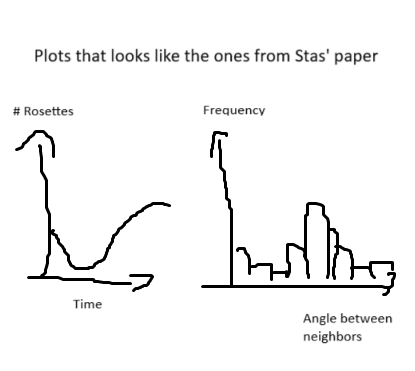
\includegraphics[width=0.8\linewidth]{chapters/Results/figures/rosettes_placeholder.png}
%     \caption{Caption}
%     \label{fig:enter-label}
% \end{figure}


\begin{figure}[H]
    \centering
    \makebox[\textwidth][c]{
    \begin{subfigure}[b]{0.55\textwidth}
    \centering
        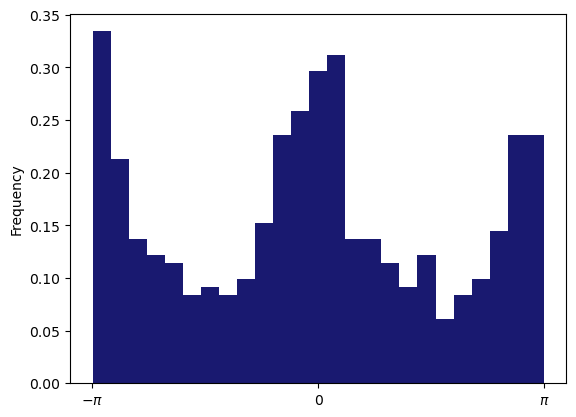
\includegraphics[width=\linewidth]{chapters/Results/figures/rosettes_angle_dist.png}

    \end{subfigure}
    \begin{subfigure}[b]{0.5\textwidth}
    \centering
    
    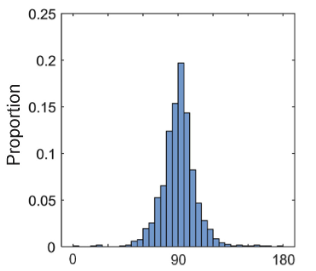
\includegraphics[width=\linewidth]{chapters/Results/figures/rosettes_angle_dist_data.png}
    \end{subfigure}
    }
    \caption{The angular distribution of the newly acquired neighbors in rosettes as found in (\textbf{left}) simulation (in radians) and (\textbf{right}) data (in degrees).}
    \label{fig:roestte-angle-dist}
    
\end{figure}
In Figure \ref{fig:roestte-angle-dist}, the distribution of angles of all found rosette-events can be seen. Strangely, the distribution is clearly bimodal in horizontal and vertical, where the ground truth has a single peak at the vertical axis. 

We believe the lack of malleability in the contours of the cells might be to blame.\\
In our model, where the equilibrium distance is the same for every direction no matter the pressure exerted, getting a bimodality is predictable.
Every time a new pair 'touch' on the up-down axis, they release space for a pair above or below on the perpendicular axis. The lack of anisotropic cell shapes almost forces this discrepancy into being.


% When speaking with Daniel, a researcher at the [Stas'] laboratory who did the original analysis, he said that this makes sense, as looking at neighboring nuclei is fundamentally different from edges. \todo{rephrase to make less bad}. 

% I won't bore you the details, so a quick run-down of our thoughts and discussions can be found in Section \ref{App:why-rosettes} in the Appendix.\\

% ... \\
% Speaking of Daniel:
% \note{
% Not showing something good :( Keep for completeness or move to appendix?}

% \subsection{Daniel-data?}
% Nothing here yet...
% \begin{figure}[H]
%     \centering
%     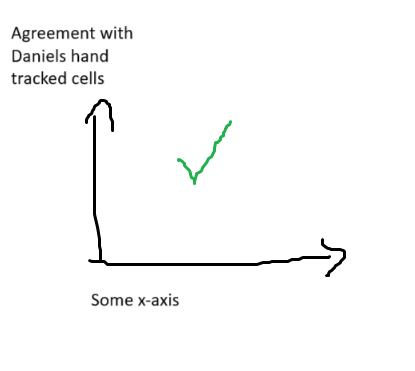
\includegraphics[width=0.7\linewidth]{chapters/Results/figures/daniel_placeholder.png}
%     \caption{Some caption}
%     \label{fig:enter-label}
% \end{figure}

% \section{Other efforts we have tried in vain}
\section{Elements cut for lack of time}
\subsection{Ventral Furrow}
We would have loved to quantify the accuracy of our simulated ventral furrow.\\
Doing computer vision cell center fit on \ref{fig:VFComparison}, for example.

\subsection{Cell surface area}
As the changes in cell surface area and percentage of invaginated tissue are known, quantifying the agreement could have helped understand the model better.

\subsection{Interaction matrix}
We have done a bunch of examinations into the mutants. combining different mutations, seeing the second-order interactions, would be an ovious and interesting next step.

\subsection{Without gene-defined PCP}
The Planar Cell Polarity was defined though the \textit{Even skipped} and \textit{Runt} stripes. Seeing the effects this had (compared to simply breaking the in-plane symmetry along the anterior-posterior axis) would have been super interesting.

